\documentclass[12pt,a4paper]{article}

\usepackage{listings}
\usepackage{xcolor}
\usepackage{graphicx}
\usepackage{hyperref}

\definecolor{codegreen}{rgb}{0,0.6,0}
\definecolor{codegray}{rgb}{0.5,0.5,0.5}
\definecolor{codepurple}{rgb}{0.58,0,0.82}
\definecolor{backcolour}{rgb}{0.95,0.95,0.92}

\lstdefinestyle{mystyle}{
	backgroundcolor=\color{backcolour},   
	commentstyle=\color{codegreen},
	keywordstyle=\color{magenta},
	numberstyle=\tiny\color{codegray},
	stringstyle=\color{codepurple},
	basicstyle=\footnotesize,
	breakatwhitespace=false,         
	breaklines=true,                 
	captionpos=b,                    
	keepspaces=true,                 
	numbers=left,                    
	numbersep=5pt,                  
	showspaces=false,                
	showstringspaces=false,
	showtabs=false,                  
	tabsize=2
}
\lstset{style=mystyle}


\title{Problem Set 3 - Solution}
\date{Due: November 12, 2021}
\author{Dino Wildi}

\begin{document}
	
	\maketitle
	
\section*{Question 1} %(20 points)}
\textit{\noindent We are interested in knowing how the difference in campaign spending between incumbent and challenger affects the incumbent's vote share. 
	\begin{enumerate}
	\item Run a regression where the outcome variable is \texttt{voteshare} and the explanatory variable is \texttt{difflog}.	
	\item Make a scatterplot of the two variables and add the regression line. 	
	\item Save the residuals of the model in a separate object.	
	\item Write the prediction equation.
\end{enumerate}
}
\lstinputlisting[language=R, firstline=7, lastline=14]{PS3_R.R}

The difference in campaign spending has a significant impact with an R-squared of 0.37, explaining a good chunk of variation but not the majority of it. This is also shown in Fig. \ref{fig:plot1}, which shows a general trend to higher vote share if there is more money spent by the incumbent compared to the challenger; and the margin of error is fairly narrow. However, we still see a pretty wide cloud of points around the regression line. The equation to predict the vote share y at any given difference in spending x is:

\[\hat{y} = 0.579 + 0.042x + e\]

\begin{figure}[h]
	\centering
	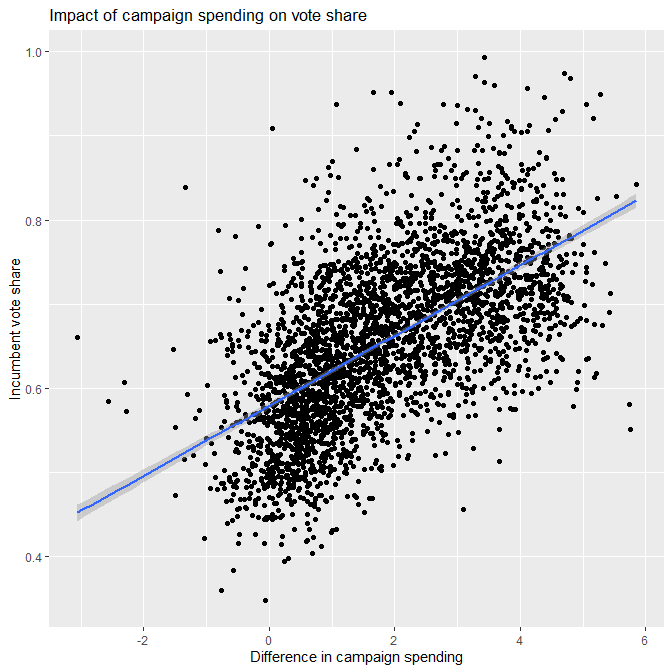
\includegraphics[width=\textwidth]{plot1}
	\caption{Impact of campaign spending on the vote share of an incumbent}
	\label{fig:plot1}
\end{figure}

\section*{Question 2}% (20 points)}
\textit{\noindent We are interested in knowing how the difference between incumbent and challenger's spending and the vote share of the presidential candidate of the incumbent's party are related.	
\vspace{.25cm}
\begin{enumerate}
	\item Run a regression where the outcome variable is \texttt{presvote} and the explanatory variable is \texttt{difflog}.
	\item Make a scatterplot of the two variables and add the regression line.
	\item Save the residuals of the model in a separate object.
	\item Write the prediction equation.
\end{enumerate}}

\lstinputlisting[language=R, firstline=20, lastline=27]{PS3_R.R}

Like above, the same relationship also holds when instead of an incumbent, we look at an incumbent party. However, it is a bit less pronounced, with the effect being smaller, as can be seen in Fig. \ref{fig:plot2}. The scatter plot is significantly more dispersed and the trend is less obvious, but still present. Likewise, the R-squared is notably lower (0.088 rather than 0.37) than in the first model using incumbents vote shares. The equation to predict the vote share of the incumbent party y at any given difference in spending x is:

\[\hat{y} = 0.508 + 0.024x + e\]

\begin{figure}[h]
	\centering
	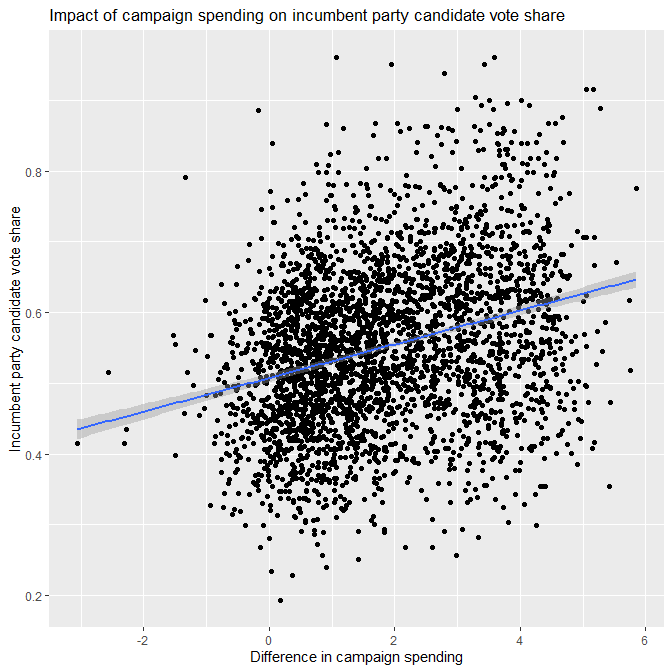
\includegraphics[width=\textwidth]{plot2}
	\caption{Impact of campaign spending on the vote share of an incumbent}
	\label{fig:plot2}
\end{figure}

\section*{Question 3}% (20 points)}
\textit{\noindent We are interested in knowing how the vote share of the presidential candidate of the incumbent's party is associated with the incumbent's electoral success.
\vspace{.25cm}
\begin{enumerate}
	\item Run a regression where the outcome variable is \texttt{voteshare} and the explanatory variable is \texttt{presvote}.
	\item Make a scatterplot of the two variables and add the regression line. 
	\item Write the prediction equation.
\end{enumerate}}

\lstinputlisting[language=R, firstline=33, lastline=39]{PS3_R.R}

This is another strong correlation, suggesting that if incumbents' parties get a high vote in the presidential election, this also increases their chance to retain their own seat. The correlation shown in Fig. \ref{fig:plot3} is relatively strong and highly significant, but does not explain all of the variation at all. The equation to predict the vote share of incumbents y at any given vote share of the incumbent's party in the presidential vote x is:

\[\hat{y} = 0.441 + 0.388x + e\]

\begin{figure}[h]
	\centering
	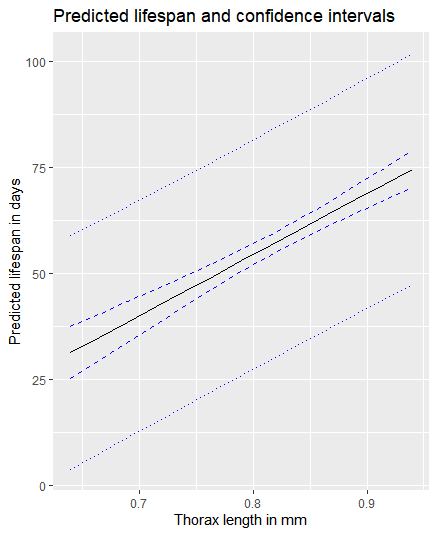
\includegraphics[width=\textwidth]{plot3}
	\caption{Impact of campaign spending on the vote share of an incumbent}
	\label{fig:plot3}
\end{figure}

\section*{Question 4}% (20 points)}
\textit{\noindent The residuals from part (a) tell us how much of the variation in \texttt{voteshare} is $not$ explained by the difference in spending between incumbent and challenger. The residuals in part (b) tell us how much of the variation in \texttt{presvote} is $not$ explained by the difference in spending between incumbent and challenger in the district.
\begin{enumerate}
	\item Run a regression where the outcome variable is the residuals from Question 1 and the explanatory variable is the residuals from Question 2.	
	\item Make a scatterplot of the two residuals and add the regression line. 	
	\item Write the prediction equation.
\end{enumerate}}

\lstinputlisting[language=R, firstline=45, lastline=51]{PS3_R.R}

The residuals are correlated to some extent, with the estimate being highly significant. This indicates that there are some unaccounted factors influencing both variables, which makes sense since factors that affect the presidential election are also likely to affect other elections taking part at the same time. Figure \ref{fig:plot4} shows that this is particularly pronounced at the high end of the range of the residuals. The prediction equation is:

\[\hat{y} = 0.257x + e\]

\begin{figure}[h]
	\centering
	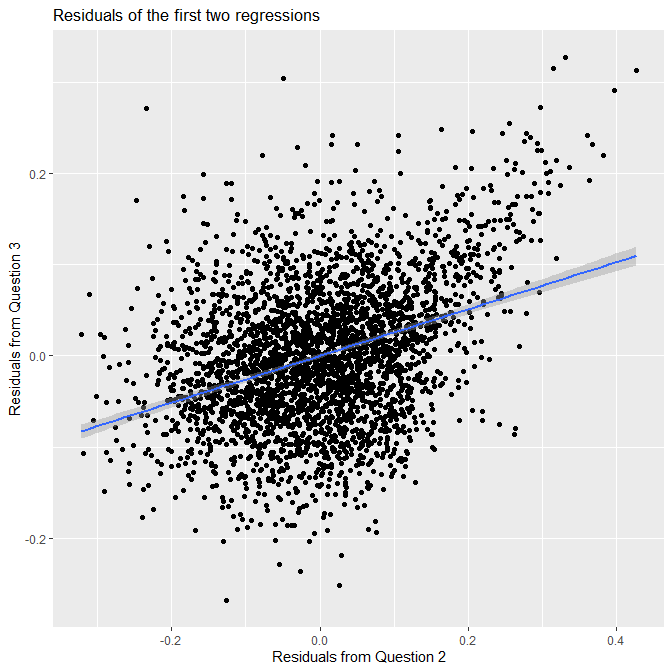
\includegraphics[width=\textwidth]{plot4}
	\caption{Impact of campaign spending on the vote share of an incumbent}
	\label{fig:plot4}
\end{figure}

\section*{Question 5}% (20 points)}
\textit{\noindent What if the incumbent's vote share is affected by both the president's popularity and the difference in spending between incumbent and challenger? 
\begin{enumerate}
	\item Run a regression where the outcome variable is the incumbent's \texttt{voteshare} and the explanatory variables are \texttt{difflog} and \texttt{presvote}.
	\item Write the prediction equation.
\end{enumerate}}

\lstinputlisting[language=R, firstline=55, lastline=56]{PS3_R.R}

The regression shows that both \texttt{difflog} and \texttt{presvote} have a significant positive effect, suggesting that both of them are related to the vote share of incumbents. The R-squared is significantly higher than in each individual regression (0.45 for both R-squared and adjusted R-squared) suggesting that this model explains more variation; once more suggesting that they are both correlated to the vote share. The prediction equation for the vote share y, predicted by the spending difference $x_{1}$ and the presidential race vote share $x_{2}$ is:

\[\hat{y} = 0.036x_{1} + 0.257x_{2} + e\]

\textit{What is it in this output that is identical to the output in Question 4? Why do you think this is the case?}

The residuals, i.e. the portion of variation not explained by the two variables, are the same as in question 4. This might be because Question 4 uses the individual residuals, i.e. unexplained variation, of \texttt{difflog} and \texttt{presvote}. Hence, by putting both variables into the same model in question 5, I expect that we explain the same variation as in Question 4, and thus also have the same residuals.

\end{document}